\chapter{Cadenas de Markov}

\section{Un modelo para redes}
En este capítulo vamos a ver cómo ordena Google las páginas que resultan de la búsqueda para mostrarlas por orden de prioridad.

Supongamos que tenemos una red de páginas web conectadas por enlaces (Google afirma cubrir unas $3\cdot 10^3$ páginas web). Vamos a ver las páginas como vértices de un grafo y los enlaces como aristas dirigidas(especificando un sentido).

Matemáticamente esto es un grafo dirigido:
\begin{center}
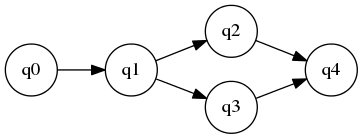
\includegraphics{tex/ejemplo_dibujo.png}
\end{center}
¿Cómo ordenar por relevancia los vértices?¿En qué orden aparecerán las páginas?


Para poder determinar que páginas son más importantes vamos a suponer un paseo aleatorio por los vértices (los internautas navegan al azar siguiendo los enlaces) de forma que una mayor acumulación en ciertos vértices indicará que son más importantes.


Aviso: No funciona literalmente, hay que hacer modificaciones.

A la larga esto converge...
\begin{center}
	\centering
	\inputtikz{grafos_mod}
\end{center}




Como había 360 al principio parece que:


\begin{itemize}
	\item Probabilidad de estar en 1 es $\frac{144}{360} = \frac{2}{5}$
	\item Probabilidad de estar en 2 es $\frac{144}{360} = \frac{2}{5}$
	\item Probabilidad de estar en 3 es $\frac{72}{360} = \frac{1}{5}$
\end{itemize}
	Según esto 1 y 2 son igual de importantes y 3 es la mitad de importante.

	La distribución que pensamos que da el límite es estacionaria (no cambia con el tiempo).



% Empieza clase del 4 de Febrero

Recordamos que en la red anterior cuando el tiempo tiende a infinito parece que la distribución de personas se estabiliza.


Parece además que sea cual sea la distribución inicial llegamos a proporciones similares. En este caso llegamos a la distribución límite $\left(\frac{2}{5},\frac{2}{5},\frac{1}{5}\right)$, que es una distribución estacionaria (no varía con el tiempo).

\section{Propiedades de los paseos aleatorios}

\textbf{¿Esta simulación con paseos aleatorios siempre sirve para ordenar los vértices (páginas web)?}

Debemos obsevar las siguientes preguntas:

\begin{itemize}
	\item ¿Existe siempre una distribución estacionaria?
	\item Si existe una distribución estacionaria ¿es única?
	\item El procedimeinto, ¿Da lugar siempre a una distribución límite?
	\item Si la distribución límite existe, ¿Es independiente de la distribución inicial?

\end{itemize}

Vamos a analizarl estas preguntas y sus respuestas una a una.

\subsection{Si existe una distribución estacionaria ¿es única?}
\label{P2}

\begin{center}
	\centering
	\inputtikz{grafosIncomunicados}
\end{center}
% nodo 4 es internet oscura

Como desde un lado de la red no se puede acceder al otro podemos decir que estas dos distribuciones son estacionarias:

$(1, 2, 3, 4, 5, 6, 7)$

$(\frac{2}{5},\frac{2}{5},\frac{1}{5}, 0, 0 , 0, 0)$ es estacionaria.

$(0, 0, 0, 0, \frac{1}{5}, \frac{2}{5}, \frac{2}{5})$ es estacionaria.


\subsection{¿Existe siempre una distribución estacionaria?}

\begin{example}{Sencillo}

	\begin{center}
		\centering
		\inputtikz{grafo3nodosSimpleTik}
	\end{center}

	Si pones todos en un nodo oscila:

	$1\; 0\; 0 \rightarrow 0\; 0\; 1 \rightarrow 0\; 1\; 0 \rightarrow 1\; 0\; 0$

	Se puede argumentar que con una distribución inicial uniforme si funciona:

	$\frac{1}{3} \; \frac{1}{3} \; \frac{1}{3} \; \rightarrow \frac{1}{3} \; \frac{1}{3} \; \frac{1}{3} \; $

	Pero esto no es verdad para cualquier grafo: partiendo de la equidistribución no se tiene la convergencia en general.

	\begin{center}
		\centering
		\inputtikz{grafo4nodosTik}
	\end{center}


	$(\frac{1}{4},\frac{1}{4},\frac{1}{4},\frac{1}{4}) \rightarrow (\frac{1}{2},\frac{1}{4},\frac{1}{4}, 0) \rightarrow (\frac{1}{4},\frac{1}{4},\frac{1}{2},0)$ oscila como antes

	\textbf{La respuesta es negativa en general}

\end{example}


\subsection {Si la distribución límite existe, ¿Es independiente de la distribución inicial?}


Basta usar como distribución inicial las distribuciones estacionarias que vimos para la segunda pregunta \ref{P2}.

\begin{obs}

Para el grafo de \ref{P2} se puede probar que $\exists$ límite:

$$(1-t)(\frac{2}{5},\frac{2}{5},\frac{1}{5},0,0,0,0) + t (0,0,0,0,\frac{1}{5},\frac{2}{5},\frac{2}{5}) \;\;\; 0 \leq t \leq 1 $$

son infinitos contraejemplos como los necesarios para la segunda pregunta \ref{P2} y la cuarta.

\end{obs}


\textbf{Spoiler} P1 es verdad y "perturbando" un poco el grafo (de manera muy sencilla) todas las preguntas tienen respuesta afirmativa.



\section{Cadenas de Markov}

\begin{defn}[Cadena de markov]
	Es una sucesión de variables aleatorias $\{X_n\}_{n=0}^{\infty}$ que toman valores en un conjunto numerable S (\textbf{conjunto de estados}) tal que
	$$Prob(X_{n+1} = V | X_n = U) = Prob(X_{n+1} = V | X_n =U , X_{n-1} = U_{n-1} , ... , X_0 = U_0)$$
	para cualesquiera $n \geq 0$ $U,V,U_0,.... ,U_{n-1} \in S$
\end{defn}


\obs Además supondremos que esta probabilidad no depende de n.


\textbf{Idea intuitiva: } n es el tiempo discretizado, lo que ocurra mañana depende con cierta probabilidad de lo que ocurre hoy sin que importe conocer la historia anterior.

Decir que no depende de n es decir que según pasa el tiempo, las reglas no cambian.

\begin{example}
	$X_n =$ suma de puntuaciones el día $n$ al tirar un dado cada día.

	El conjunto de todos los estados serían todas las puntuaciones posibles . (S = naturales)

	Sabiendo lo que llevo acumulado hoy, tengo una cierta probabilidad de obtener mañana diferentes resultados, pero no depende de lo que ocurrió ayer; no me importa cómo he llegado a sumar lo que llevo hoy.
\end{example}

\begin{example}[2]
	S = puntuaciones en el tenis.\\
	$X_n =$ puntuación el en punto n\\
	Suponemos que el jugador A tiene prob $p > 1/2$ de ganar cada punto.\\
	Pensando un poco las puntuaciones en el tenis vemos que S solo puede tener 20 elementos.\\
	S= puntuaciones numéricas, deuce, advantages(A o B) , victoria (A o B).\\
	Se puede comprobar que:
	$$Prob(\text{victoria A}) = \frac{p^4 \cdot(1- 16(1-p)^4)}{p^4 - (1-p)^4}$$
	Esto es como curiosidad, ver que con tener sólo un poco más de probabilidad de ganar un punto, la probabilidad de ganar un juego y un set va creciendo.
\end{example}




Si $|S| = \infty$ entonces la cadena de Markov es infinita y se supone $S = \ent^+ (\nat -\{0\})$


Si $|S| < \infty$ entonces la cadena de Markov es finita y se supone $S =\{1,2,...,N\}$

\begin{defn}[Probabilidad de transición]
	del estado i al j
	$$P_{ij} = Prob(X_{n+1} = j| X_n = i) = Prob (X_1 = j| X_0 = i)$$
\end{defn}

Los $P_{ij}$ forman la \textbf{matriz de transición}.

\newpage
\textbf{Propiedades}
\begin{enumerate}
	\item $\sum_{j \in S} P_{ij} = 1$
	\item $Prob(X_1 = j)= \sum_{i \in S} Prob(X_0 = i)P_{ij}$\\
\end{enumerate}

\begin{proof}
	\begin{enumerate}
		\item $\sum_{j \in S} P_{ij} = \sum_{j\in S} Prob(X_1 = j | X_0 = i) = Prob (X_1 \in S | X_0 = i) = 1$
		\item Utilizando la ley de la probabilidad total

		$$Prob(X_1 = j) = \sum_{i \in S} Prob (X_0 = i) \cdot Prob(X_1 = j| X_0 = i)$$
	\end{enumerate}
\end{proof}

	\begin{defn}[Ley de la probabilidad total]
		Sea  $\{A_1, A_2,...,A_n\}$ una partición de $\Omega$ con $P(A_i)>0 \forall i=1,2,...,n$. Entonces, $\forall B \subset \Omega$ medible (perteneciente a $\algb{M}$):
		\[
		P(B)=\sum_{i=1}^{n}P(B\cap A_i)=\sum_{i=1}^{n}P(B|A_i)P(A_i)
		\]
		Esta propiedad se obtiene de despejar de la formula de la probabilidad condicionada:
		\[P(A|B)=\frac{P(A \cap B)}{P(B)}\]
	\end{defn}


De las dos propiedades deducimos que:
\begin{itemize}
	\item \textbf{(prop.1)} La matriz de transición $P_{ij} i,j \in S$ tiene elementos $0 \leq P_{ij} \leq 1$ y la suma de los elementos de cada fila es 1.
	\item Escribiendo ($\prod_0$) = ${Prob (X_0 =i)}_{i \in S}$ como vector fila, y ($\prod_n$) = ${Prob (X_n =i)}_{i \in S}$

	Entonces por \textbf{(prop.2)} : ($\prod_0$) $ = (\prod_n)\cdot P$ (P = matriz de transición)
\end{itemize}

De la misma forma $(\prod_2) = (\prod_1) \cdot P$, etc...

Iterando nos queda:
$$\left(\prod_n\right) = \left(\prod_0\right) \cdot P^n$$

Ahora vemos cómo aplicar esto a las páginas web.


Teniendo en cuenta que en la realidad la P sería una matriz de $3\cdot 10^{13} \times 3\cdot 10^{13}$ la forma más fácil de calcular $P^n$ es con la forma canónica de Jordan. Veámoslo con un ejemplo.
\begin{example}[1]{}

%Hola kasner, tienes dos opciones, la que creo que quieres es la que no está comentada, q es la que está justo despues de la comentada. Ala, me debes un café.

%\begin{figure}[ht]
%	\centering
%	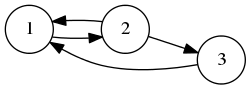
\includegraphics{tex/grafo3nodos.png}
%	\caption{Figurita molona}
%\end{figure}

	\begin{center}
	\centering
	\inputtikz{grafo3nodosTik}
\end{center}


	S= páginas web (vértices)\\
	$P_{ij}$ = probabilidad de , estando en la página i, llegar a la página j en el instante siguiente.

	$$Prob(X_1 = (2)| X_0 = (1)) = 1$$
	$$P =\left(\begin{matrix}
	0 & 1 & 0\\
	1/2 & 0 & 1/2\\
	1 & 0 & 0
	\end{matrix}\right)$$

	Hacemos Jordan:
	$$P = C^{-1} \left(\begin{matrix}
	1&&\\
	&z&\\
	&&\overline{z}
	\end{matrix}\right) C$$
	Haciendo los cálculos nos queda $z = \frac{1}{\sqrt{2}}\cdot e^{\frac{3\pi i}{4}}$

	Por lo tanto:
	$$P^n =  C^{-1} \left(\begin{matrix}
	1&&\\
	&z^n&\\
	&&\overline{z}^n
	\end{matrix}\right) C \stackrel{n\rightarrow \infty}{\rightarrow}  C^{-1} \left(\begin{matrix}
	1&&\\
	&0&\\
	&&0
	\end{matrix}\right) C = \left(\begin{matrix}
	2/5&2/5&1/5\\
	2/5&2/5&1/5\\
	2/5&2/5&1/5
	\end{matrix}\right) = L$$
	Esto implica que:
	$$\lim_{n\rightarrow\infty}(\prod_n) = \lim_{n\rightarrow\infty}(\prod_0)\cdot P^n = (\prod_0)\cdot L =( \begin{matrix}
	2/5&2/5&2/5
	\end{matrix})$$
	Que es independiente de $\prod_0$
\end{example}

\begin{example}[2]

	\begin{center}
		\centering
		\inputtikz{grafo4nodosTik}
	\end{center}

	$$P = \left( \begin{matrix}
	0 & 1 & 0 & 0\\
	0 & 0 & 1 & 0\\
	1 & 0 & 0 & 0\\
	1 & 0 & 0 & 0\\
	\end{matrix}\right)= C^{-1} \left(\begin{matrix}
	1&&&&\\
	&w&&&\\
	&&\overline{w}&\\
	&&&0
	\end{matrix}
	\right)\cdot C$$
	$w = e^{\frac{2\pi i}{3}}$ , si seguimos calculando las potencias de $w$ y de $\overline{w}$ vemos que van oscilando entre los valores $w , \overline{w} , 1$, por lo que vemos que en este caso $P^n$ no tiene límite.
	$$\exists\left(\prod_0\right) : \nexists \lim \left(\prod_0\right)\cdot P^n$$
	Sin embargo con $(\prod_0) = (\begin{matrix}
	1/3&1/3&1/3&0
	\end{matrix}) $ se comprueba $(\prod_0) = (\prod_0)\cdot P$


	Con lo que para ese $(\prod_0)$ si tenemos límite.Ya veremos más adelante cómo se llaman este tipo de distribuciones.
\end{example}

Lo que hemos comprobado con estos dos ejemplos es que si conocemos la forma canónica de Jordan podemos saber si tenemos convergencia o no.

\paragraph{Resumen de lo visto hasta ahora}
\begin{itemize}
	\item Cadenas de Markov $\begin{cases}
	(\prod_0) = \{P(X_0 = i)\}_{i \in S} \rightarrow \text{\textbf{distribución inicial}}\\
	P = \text{Matriz de transición}
	\end{cases}$
	\item Distribución de probabilidad en el instante 0 = $(\prod_0)P^n$
	\item $P^n$ se calcula con la forma canónica de Jordan
	\item En general nos queremos que exista la \textbf{distribución límite} : $\lim_{n\rightarrow\infty} (\prod_0) P^n$
\end{itemize}

\obs Si existe $(\prod) = \lim (\prod_0) P^n$ entonces $(\prod) = (\prod) P$
\begin{proof}
	$(\prod) = \lim(\prod_0) P^{n+1} = (\lim (\prod_0)P^n)P = (\prod) P$
\end{proof}

\begin{defn}[Distribuciones estacionarias]
	Se dice que $(\prod)$ es una distribución de probabilidad estacionaria si:
	$$(\prod)\cdot P = (\prod)$$
\end{defn}

\obs Con estas distribuciones podemos calcular el límite y estudiar la convergencia sin utilizar la forma canónica de Jordan.


Recordando las preguntas que nos hicimos con las propiedades de los paseos aleatorios vemos que, experimentalmente, las cadenas de Markov muy interconectadas responden afirmativamente a estas preguntas.

Vamos a ver dos versiones de lo que se entiende por \textbf{conexión} de una cadena de Markov
\newpage
\begin{itemize}
	\item \begin{defn}[Irreducible]
		Se dice que una cadena de Markov es \textbf{irreducible} si se puede ir de un estado a otro en un número finito de pasos. Es decir
		$$\forall i,j \in S\text{    }\exists k : P(X_k = j| X_0 = i) \neq 0$$
		Otra forma de definirlo es con la matriz de transición:
		$$\forall i,j \in S \text{    }\exists k: (P^k)_{ij} \neq 0$$
	\end{defn}
	\item \begin{defn}[Regular]
		Se dice que una cadena de Markov es \textbf{regular} si existe un número de pasos tal que dándolos se puede pasar de un estado a cualquier otro. Es decir:
		$$ \exists k : P(X_k = j| X_0 = i) \neq 0  \forall i,j \in S $$
		Otra forma de definirlo es con la matriz de transición:
		$$\exists k : \text{ todos los elementos de} P^k \text{ son positivos.}$$
	\end{defn}
\end{itemize}


Experimentos: mucha "interconexión" $\rightarrow$ $\exists \lim (\Pi_0)P^n$ y no depende de $(\Pi_0)$.

En principio sabemos resolver cada problema, en caso finito, con la forma canónica pero esto no es muy práctico.

\begin{theorem}{Teorema 1}
	\label{Markov_tma1}
	Una cadena de Markov finita siempre tiene al menos una distribución estacionaria.
\end{theorem}

\begin{theorem}{Teorema 2}
	\label{Markov_tma2}
	Para una cadena de Markov finita regular $\exists \lim (\Pi_0) P^n$ y el resultado no depende de $(\Pi_0)$ y es la única distribución estacionaria.
\end{theorem}

\begin{theorem}{Teorema 3}
	\label{Markov_tma3}
	Para cualquier cadena de Markov finita, el límite:
	\[\lim \frac{(\Pi_0)+(\Pi_1)+…+(\Pi_n)}{n+1}  \text{ (con }(\Pi_n) = (\Pi_0)P^n\text{)}\]
	existe y converge a una distribución estacionaria.
\end{theorem}


\begin{example}

\begin{figure}[hbtp]
	\centering
	\inputtikz{markov/triangulos_separados}
\end{figure}

Tenía muchas distribuciones estacionarias: $\exists \lim(\Pi_0)P^n$ pero depende de $(\Pi_0)$.

No es irreducible $\Rightarrow^{\text{(lo veremos)}}$ se pierde la unicidad de la distribución estacionaria.

\end{example}

\begin{example}

\begin{figure}[h!btp]
	\centering
	\inputtikz{markov/triangulo_con_entrada}
\end{figure}

No es regular, por ello hay dependencia en $(\Pi_0)$, no es regular, no existe $\lim(\Pi_0) P^n$ en general. Pero $\exists \lim$ del tercer teorema \ref{Markov_tma3} y en $(\frac{1}{2},\frac{1}{3},\frac{1}{3},0)$.

\end{example}


\subsection{Page Rank Algorithm}

\begin{figure}[hbtp]
	\centering
	\inputtikz{markov/red_pagerank}
\end{figure}


$$\text{Modelo: } P_y = \left\{
	\begin{array}{ll}
		0  & \mbox{si} \text{no hay enlace de i a j} \\
		\frac{1}{\text{nº de enlaces salientes}} & \mbox{si} \text{hay enlace de i a j}
	\end{array}
\right.
$$

P es una matriz $N \times N$ $N = 3 \, 10^{13}$.

\textbf{Idea} Si estuviéramos en las hipótesis del Tma 2 \ref{Markov_tma2} entonces  $(\Pi_0) P^{\text{nº grande}}$ aproximaría la distribución de probabilidades de estar en cada página (navegando por los enlaces al azar) (en la práctica $50 \leq \text{nº grande} \leq 100$).


Esencialmente lo que se hace para estar las hipótesis del Tma 2 \ref{Markov_tma2} es cambiar ceros por números pequeños.
$\Rightarrow P$ se vuelve una matriz con elementos $> 0$.
$\Rightarrow$ se cumple la definición de regular con $k=1$.

Concretamente se cambia la $P$ original por:

$$P_{\epsilon} = (1-\epsilon) P + \epsilon E \;\;\;\; E = \text{matriz con todos sus elementos } \frac{1}{n}$$

\begin{example}

\begin{figure}[hbtp]
	\centering
	\inputtikz{markov/grafo_2-ciclo}
\end{figure}

	$$P = \left( \begin{array}{ccc}
0 & 1 & 0 \\
0 & 0 & 1 \\
0 & 1 & 0 \end{array} \right)$$

$0 \rightarrow \epsilon$ no es posible porque no sumarían 1 las filas.



$$P_{\delta} = \left( \begin{array}{ccc}
\delta & \;\; 1-2\delta \;\; & \delta \\
\delta & \;\; \delta \;\;& 1 - 2 \delta\\
\delta & \;\; 1 - 2 \delta \;\; & \delta \end{array} \right)$$

$0 \rightarrow \delta$ y ajusto los elementos no nulos para que sumen 1.


$\delta = \frac{\epsilon}{3}$ (solo notación) $\Rightarrow$ esta última matriz es:


$$= (1-\epsilon)\left( \begin{array}{ccc}
0 & 1 & 0 \\
0 & 0 & 1 \\
0 & 1 & 0 \end{array} \right) + \epsilon \left( \begin{array}{ccc}
1/3 & 1/3 & 1/3 \\
1/3 & 1/3 & 1/3 \\
1/3 & 1/3 & 1/3 \end{array} \right)$$


Es facil comprobar (ej) que $P_{\epsilon}$ tiene filas con suma 1. Además, si $\epsilon$ pequeño, $P_{\epsilon} ≈ P$.

Lo que hacen los $\epsilon$ es representar la posibilidad de que alguien salte a una página aleatoria.

\begin{figure}[hbtp]
	\centering
	\inputtikz{markov/grafo_2-ciclo_completo}
\end{figure}

\end{example}